\section{Analysis strategy}
The search targets the $H^+$ production decaying into $tb$ in the single-lepton channel. The events that pass the selection described in Section~\ref{Hplustb:SectionEventSelection} are further divided into two types of disjointed analysis regions: signal regions and control regions. The control regions are used to improve the modelling of the \ttbar+jets background. Furthermore, several multi-variate techniques are used to improve the separation between signal and background events.

\subsection{Region definition}

The analysis regions are categorised as a function of the number of reconstructed jets and $b$-tagged jets at the 70\% $b$-tagging WP. The signal regions are 5j3b, 5j$\geq$4b, $\geq$6j3b and $\geq$6j$\geq$4b. Figure~\ref{Hplustb:cheeseplots} illustrates the background composition, which clearly shows the dominance of the \ttbar\ background, specially the \ttb\ component in the $\geq$4b regions. The 3b categories consist of a mixture of the three \ttbar\ components: 52\% of the 5j3b background are \ttl\ events, while the 70\% of the $\geq$6j3b events is split equal by \ttb\ and \ttl\ events.

\begin{figure}[htbp]
    \RawFloats
    \begin{center}
    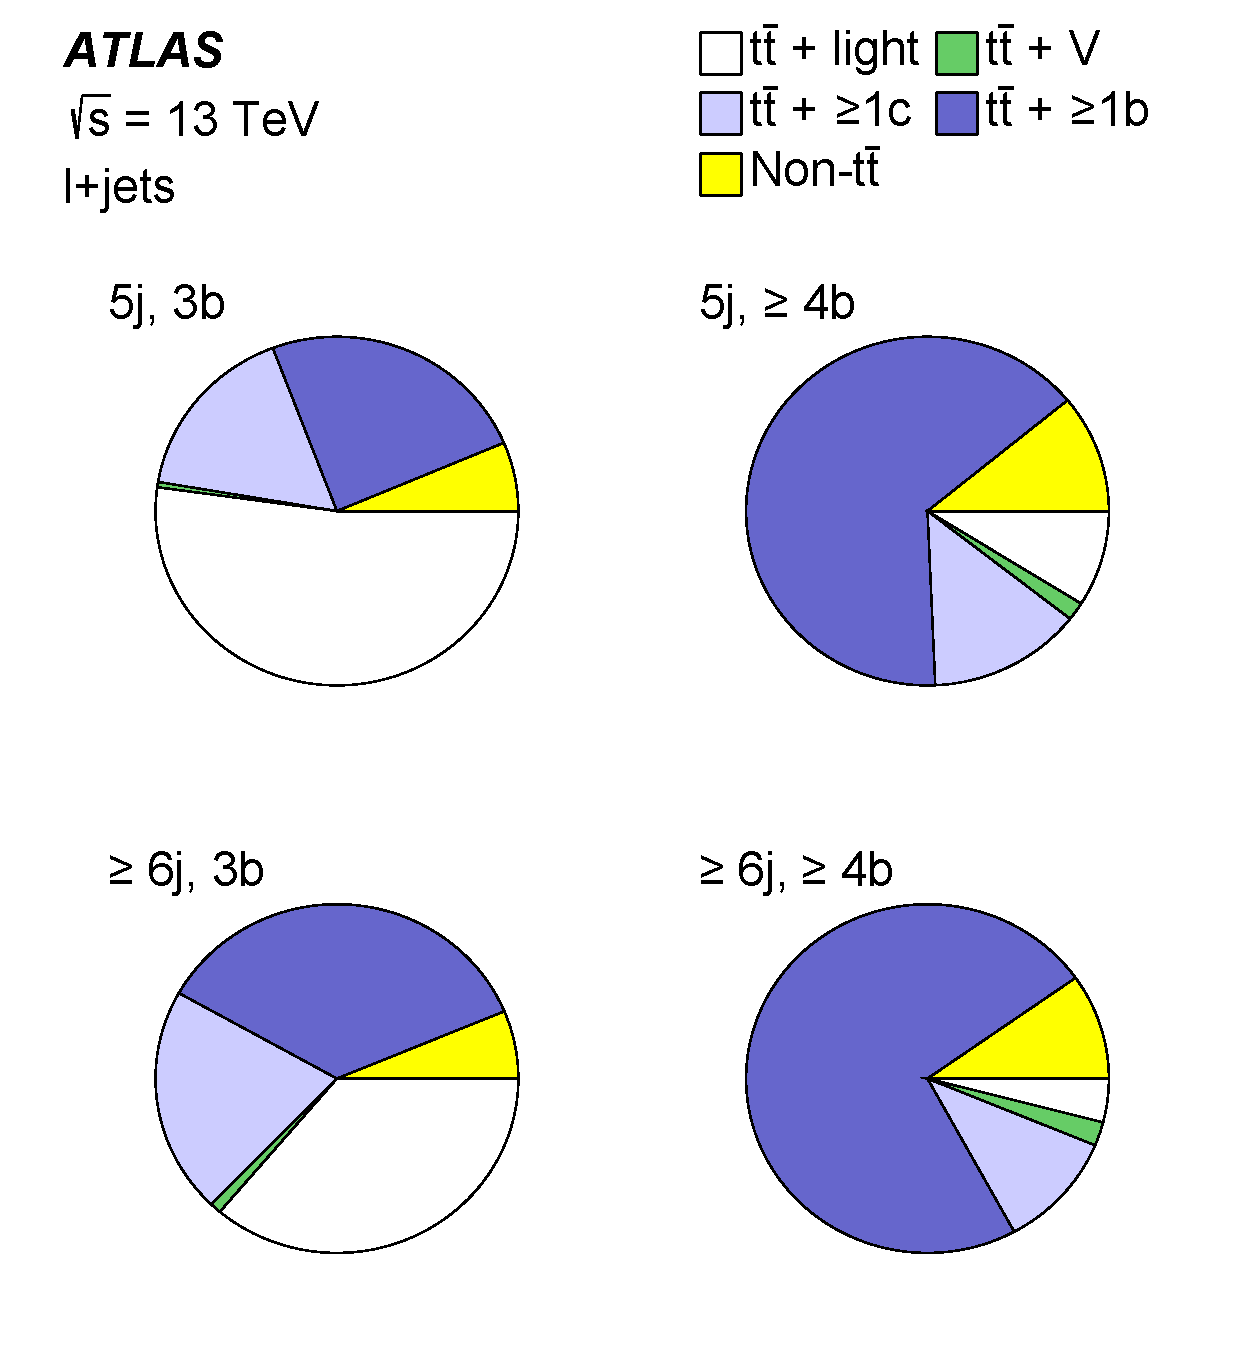
\includegraphics[width=0.75\textwidth]{HPLUSTB/cheeseplot.pdf}
    \caption{
        Background composition in the various analysis regions.
    }
    \label{Hplustb:cheeseplots}
    \end{center}
\end{figure}

Table~\ref{Hplustb:prefityields} shows the number of expected and selected events in the different regions, including the $\geq$5j2b selection which is used to derive weights to improve the background modelling, as shown in the next section. The number of expected $H^+$ signal events for the 600 GeV mass hypothesis is also shown, which is only contribution is less than 0.5\% for the $\geq$5j2b and thus considered negligible. Another observation, is that the region with the higher sensitivity in terms of $n_S/\sqrt{n_B}$ is the $\geq$ 6j$\geq$ 4b region  %Table 6 shows the cut flow for each signal sample.

\begin{table}[htb]
    \small
    \addtolength{\leftskip} {-4cm} % menja marges
    \addtolength{\rightskip}{-4cm}
    \centering
    \begin{tabular}{l r r r r r}
        \toprule\toprule
          & $\geq$ 5j, 2b & {5j, 3b} & {5j, $\geq$ 4b} & {$\geq$ 6j, 3b} & {$\geq$ 6j, $\geq$ 4b}\\
          \midrule 
  $t\bar{t}$ + light        & 1365450 $\pm$ 420 & 44000 $\pm$ 8000  & 290 $\pm$ 130  & 31000 $\pm$ 6000  & 340 $\pm$ 180 \\ 
  $t\bar{t}$ + $\geq$1$b$   & 92380   $\pm$ 44 & 20500  $\pm$ 2400  & 2080 $\pm$ 240 & 30000 $\pm$ 4000  & 6100 $\pm$ 1500   \\ 
  $t\bar{t}$ + $\geq$1$c$   & 217830  $\pm$ 120 & 14000 $\pm$ 1600  & 440 $\pm$ 90   & 17800 $\pm$ 2400  & 910  $\pm$ 180   \\ 
  $t\bar{t}$ + $W$          & 3181    $\pm$ 5   & 109   $\pm$ 16    & 3.2 $\pm$ 0.6  & 230   $\pm$ 40    & 15.7   $\pm$ 2.8 \\ 
  $t\bar{t}$ + $Z$          & 3976    $\pm$ 12  & 300   $\pm$ 40    & 51  $\pm$ 7    & 650   $\pm$ 90    & 169  $\pm$ 24 \\ 
  $Wt$ channel              & 46190   $\pm$ 110 & 2300  $\pm$ 600   & 80  $\pm$ 50   & 1800  $\pm$ 800   & 150  $\pm$ 90 \\ 
  $t$ channel               & 19505   $\pm$ 74  & 790   $\pm$ 310   & 55  $\pm$ 21   & 600   $\pm$ 500   & 70   $\pm$ 50 \\ 
  Other top         & 1898    $\pm$ 8   & 125   $\pm$ 17    & 17.7  $\pm$ 3.3    & 190   $\pm$ 70    & 60   $\pm$ 24 \\ 
  $VV$ \& $V$ + jets        & 49830   $\pm$ 140 & 1700  $\pm$ 700   & 68  $\pm$ 25   & 1600  $\pm$ 600   & 120  $\pm$ 50 \\ 
  $t\bar{t}H$               & 2918    $\pm$ 2   & 530   $\pm$ 60    & 129 $\pm$ 20   & 1110  $\pm$ 130   & 420  $\pm$ 60 \\ 
\midrule      
  Total                     &1803170 $\pm$ 480 & 84000 $\pm$ 10000 & 3200$\pm$ 400 & 85000 $\pm$ 12000 & 8400 $\pm$ 1700 \\
\midrule
  Data                      &1830756           & 95852             & 4109          & 98929          & 10552 \\
\midrule  
\midrule\ 600 GeV             & 1911 $\pm$ 24   & 520 $\pm$ 40      & 73 $\pm$ 8    & 960 $\pm$ 80   & 279 $\pm$ 25  \\   
\bottomrule\bottomrule                               
    \end{tabular}
    \caption{Number of expected and selected events split according to the analysis regions. The $\geq$ 5j, 2b region is used to derive weights to improve the data/simulation agreement. The quoted uncertainties include both statistical and systematic uncertainties except for the first column ($\geq$ 5j, 2b) which only includes statistical uncertainties. The predicted number of $H^+$ signal events for the 600 GeV mass hypothesis is also shown, assuming a cross-section times branching fraction of 0.32~pb.}
    \label{Hplustb:prefityields}
\end{table}

Figure~\ref{Hplustb:acceptance} shows the acceptance times efficiency of the $\geq$5j$\geq$3b inclusive selection per signal mass sample. It can be observed the decrease in acceptance starting from 1000~GeV due to the loss of jets, characteristic of boosted regimes.

\begin{figure}[htbp]
    \RawFloats
    \begin{center}
    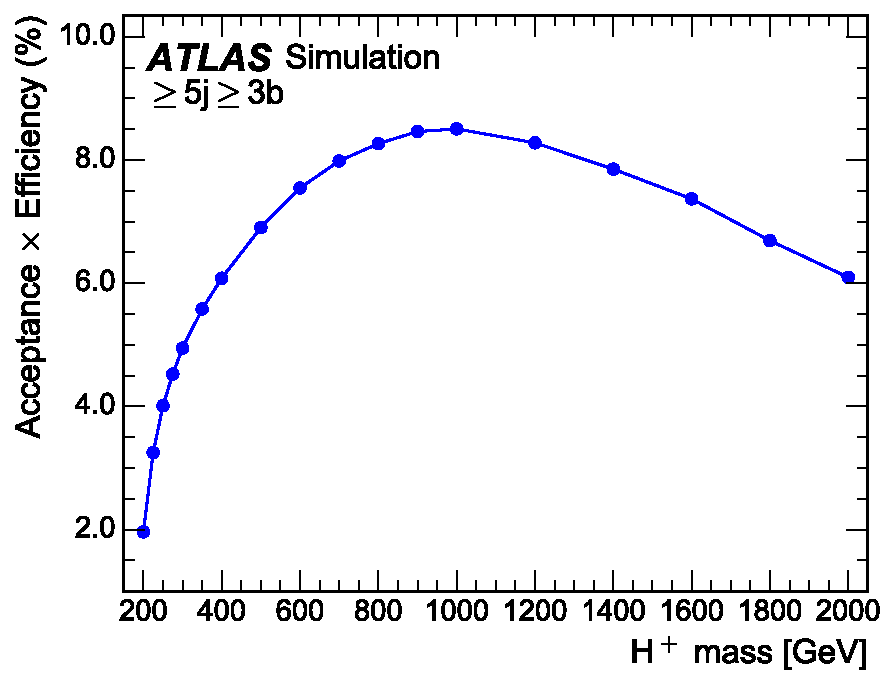
\includegraphics[width=0.75\textwidth]{HPLUSTB/acceptance.pdf}
    \caption{
        Total event acceptance of every $H^+$ signal sample. Statistical uncertainties are included but hidden within the markers.
    }
    \label{Hplustb:acceptance}
    \end{center}
\end{figure}

\clearpage
\subsection{Reweighting technique}
\label{Hplustb:secRW}
The main background for the search is \ttbar+jets, and its correct modelling is essential for the correct description of the data. It is observed that the simulation does not properly model high jet multiplicities nor the hardness of additional jet emissions %https://cds.cern.ch/record/2630327 https://link.springer.com/article/10.1007/JHEP01(2021)033
To improve the data/MC agreement of this essential background, data-based corrections are applied to the \ttbar samples. Since the mismodelling is assumed to be due mainly to the additional radiation in the parton shower, hence independent on the flavour of the associated jets, the corrections derived in the $\geq$5j2b regions are expected to improve the agreement in the 3b and $\geq$4b regions. The remaining discrepancies can still be covered by the systematic model.

The corrections are derived for each jet multiplicity and as a function of \HTall, defined as the scalar \pT sum of jets and the lepton, i.e. all the selected objects. The reweighting factors for each jet multiplicity is expressed as:

\begin{equation}
    \label{Hplustb:RWeq}
    R(\HTall)=\frac{ Data(\HTall) - \text{MC}^{\text{non-\ttbar}(\HTall)} }{\text{MC}^{\text{\ttbar}(\HTall)}}
\end{equation}

and, by construction, assumes that any disagreement between data and MC is from \ttbar. In this context, \ttbar\ includes \ttb, \ttc\ and \ttl\ as well as single top $tW$ contributions. 

Figure~\ref{Hplustb:RWfactors} includes all the derived corrections, showing higher weights for increased jet multiplicities and, in general, the \HTall corrections have a hyperbolic behaviour: converging $\HTall > 800$~GeV and rapidly increasing towards lower values. Among various functions tried, the hyperbola plus a sigmoid functional form was found to be the best fit to the \HTall weight distributions: $w=a+\frac{b}{(\HTall)^c} - \frac{d}{1+\exp(e-f\cdot\HTall)}$. The eigenvalues of the error matrix of fitted parameters are included as systematic uncertainties. 

\begin{figure}[htb]
    \RawFloats
    \begin{center}
    \subfloat[$\ge$5j2b]{\includegraphics[width = 0.5\textwidth]{HPLUSTB/Reweighting/nominal_jets.pdf}} \\ 
    \subfloat[5j2b]{\includegraphics[width = 0.5\textwidth]{HPLUSTB/Reweighting/fitparsvar_hyp_5j.pdf}} 
    \subfloat[6j2b]{\includegraphics[width = 0.5\textwidth]{HPLUSTB/Reweighting/fitparsvar_hyp_6j.pdf}}  \\
    \subfloat[7j2b]{\includegraphics[width = 0.5\textwidth]{HPLUSTB/Reweighting/fitparsvar_hyp_7j.pdf}}
    \subfloat[$\ge$8j2b]{\includegraphics[width = 0.5\textwidth]{HPLUSTB/Reweighting/fitparsvar_hyp_8j.pdf}}
    \caption{Reweighting factors (weights) obtained from the comparison between data and simulation of the number of jets (a) and \HTall\ for various jet multiplicity selections (b) to (e).
    The errors in the data points include the statistical uncertainties in data and MC predictions.}
    \label{Hplustb:RWfactors}
\end{center}
\end{figure}

The agreement between simulation and data in the analysis region improves, as an example, Figure~\ref{Hplustb:RWeffect} shows the improvement in the leading jet \pT\ distribution before and after the reweighting. The remaining disagreement is specially from normalisation effects. All figures included in this document are shown after the reweighting corrections are applied, unless stated otherwise

\begin{figure}[htb]
    \RawFloats
    \begin{center}
    \subfloat[5j3b, unweighted]
    {\includegraphics[width = 0.33\textwidth]{HPLUSTB/Reweighting/unrw/plot_5jex3bex_jet_pt.pdf}}
    \subfloat[5j3b, reweighted] 
    {\includegraphics[width = 0.33\textwidth]{HPLUSTB/Reweighting/rw/plot_5jex3bex_jet_pt.pdf}} \\
     \subfloat[5j$\ge$4b, unweighted]
    {\includegraphics[width = 0.33\textwidth]{HPLUSTB/Reweighting/unrw/plot_5jex4bin_jet_pt.pdf}} 
     \subfloat[5j$\ge$4b, reweighted]
    {\includegraphics[width = 0.33\textwidth]{HPLUSTB/Reweighting/rw/plot_5jex4bin_jet_pt.pdf}}  \\
     \subfloat[$\ge$6j3b, unweighted] 
    {\includegraphics[width = 0.33\textwidth]{HPLUSTB/Reweighting/unrw/plot_6jin3bex_jet_pt.pdf}} 
     \subfloat[$\ge$6j3b, reweighted] 
    {\includegraphics[width = 0.33\textwidth]{HPLUSTB/Reweighting/rw/plot_6jin3bex_jet_pt.pdf}} \\ 
     \subfloat[$\ge$6j$\ge$4b, unweighted]
    {\includegraphics[width = 0.33\textwidth]{HPLUSTB/Reweighting/unrw/plot_6jin4bin_jet_pt.pdf}} 
     \subfloat[$\ge$6j$\ge$4b, reweighted]
    {\includegraphics[width = 0.33\textwidth]{HPLUSTB/Reweighting/rw/plot_6jin4bin_jet_pt.pdf}} \\  
    \caption{Comparison of the predicted leading jet \pT\ and data before the fit in the four analysis regions before (left) and after (right) the reweighting was applied. The uncertainty bands include both the statistical and systematic uncertainties, except for the cross-sections of the \ttb\ and \ttc\ backgrounds.
    The lower panels display the ratio of the data to the total prediction. 
    The hatched bands show the uncertainties before the fit to the data,  which are dominated by systematic uncertainties. The $\chi^2/\mathrm{ndf}$ and the $\chi^2$ probability are also shown. Statistical uncertainties on MC predictions and data are uncorrelated across bins, while systematic uncertainties on the predictions are correlated.}
    \label{Hplustb:RWeffect}
\end{center}
\end{figure}
\clearpage
\subsection{Multivariate techniques}

Multivariate techniques are used in this analysis to enhance the separation between signal and background. The kinematics of \ttb\ and signal events are very similar, and these methods can use different distributions as inputs to obtain a powerful discriminating variable. The main classificator is a parameterised NN trained over all signal and background. As an input variable, a kinematic discriminant is used to enchance the separation between the a $H^+$ sample and \ttbar + jets.

\subsubsection{$H^+$ parameterised NN}

A set of NNs is trained for each of the signal regions: 5j3b, 5j$\geq$4b, $\geq$6j3b and $\geq$6j$\geq$4b separately. The NN uses high-level variables as input, hence a simple and small architecture is enough to extract all the discrimination power: the architecture is sequential with two fully connected layers of 64 nodes and a single output node, and is implemented with the Python deep learning library, Keras\todo{tocite}. The activation function used is the commonly employed "rectified linear unit", the loss is the "binary cross-entropy" function and the optimiser is the Adam algorithm. Batch normalisation is performed to speed up the learning process, dropout is applied during training at a 10\% rate. To further regularise the training, inputs are transformed to the same scale (same mean and variance) as the training set, event weights of each label add up to the same value and a two-fold cross-validation setup is used. All signal samples are used in the training against all background samples, which are weighted according to their cross-sections. Table~\ref{Hplustb:inputNNtable} shows the 15 variables used as input for the NN, which includes the $H^+$ mass. The NN that uses this technique, normally referred as parameterised NN, is being provided with an input that distinguishes the different signals and has the output as a function of the $H^+$ value\todo{tocite}. For signal events the parameter corresponds to the mass of the $H^+$, while for background events a random value of the $H^+$ is assigned to each event, taken from the distribution of signal masses. This makes the NN not to directly use the parameter to perfectly classify the events.

\begin{table}[htb]
    \centering
    \small
    \begin{tabular}{l l}
        \toprule\toprule
        \multicolumn{1}{c}{Variable}  &  \multicolumn{1}{c}{Description}  \\
        \midrule
        $m_{H^+}$               & Parameter of the NN. $H^+$ mass hypothesis. \\
        $D$                     &   Kinematic discriminant of the $H^+$ mass hypothesis.   \\
        \HTjets &   Scalar sum of the transverse energy of all jets. \\
        &  Sensible to events with massive $H^+$  \\
        Centrality         &   Centrality calculated using all jets and leptons.   \\
        $\pT^0$                 &   Leading jet \pT. Similar to \HTjets. \\
        $m^{\text{min}\Delta R}_{bb}$     &   Invariant mass of the closest $b$-jet pair. \\
        &                                     The $bb$ pair aims to partially reconstruct the $H^+$ invariant mass,\\
        &                                      very different from the \ttbar\ background. \\
        $\pT^4$  &   \pT of fifth leading jet. Characterises the low energy scale of the event.  \\
        $H_1^{\mathrm{all}}$    &   Second Fox-Wolfram moment calculated using all jets and leptons.  \\ %https://journals.aps.org/prd/abstract/10.1103/PhysRevD.87.073014
        $\Delta R^{\text{avg}}_{bb}$ &   Average $\Delta R$ between all $b$-jet pairs in the event. \\
        $\text{min}\Delta R_{lep,bb}$  &   $\Delta R$ between the lepton and the pair of $b$-jets with smallest $\Delta R$.   \\
        $m^{\text{min}\Delta R}_{uu}$   &   Invariant mass of the untagged jet-pair with minimum $\Delta R$.\\
                                        &  Aims to reconstruct the $W$-boson that decays hadronically.   \\
        $m^{\text{max}\pT}_{bb}$ &   Invariant mass of the $b$-jet pair with maximum \pT.  \\
        $m^{\text{max}m}_{bb}$  &   Maximal invariant mass of $b$-jets.   \\
        $m^{\text{max}\pT}_{jjj}$ &   Invariant mass of the jet triplet with maximum \pT.  \\
        $N_{\text{jets}}$ and $N_{b\text{-jets}}$ & jet and $b$-jet multiplicity. \\
        \bottomrule\bottomrule
        \end{tabular}
    \caption{List of variables included in the training of the NN.}
    \label{Hplustb:inputNNtable}
\end{table}

The kinematic discriminant, \HTjets, the centrality and the leading jet \pT\ are consistently among the most important variables in the four analysis regions. The NN output is obtained evaluating the NN setting the $H^+$ at the desired hypothesis. The obtained distributions for signal and background in the analysis regions for the 200 and 800~GeV $H^+$ masses are shown in Figure~\ref{Hplustb:NNshapes}. The shapes are significantly different between the two mass-points, although the shape of the distributions transforms gradually from one mass to the next. Notice that the shape of the background changes, since the same NN is being evaluated but with a different $H^+$ mass value. The separation of the $H^+$ signal from the background is most difficult for low $H^+$ masses because the two processes have very similar kinematics and topology.

\begin{figure}[htb]
    \RawFloats
    \centering
    \subfloat[5j3b]{\includegraphics[width = 0.5\textwidth]{HPLUSTB/NNshapes/INC_5j3b_200.pdf}} 
    \subfloat[5j$\ge$4b]{\includegraphics[width = 0.5\textwidth]{HPLUSTB/NNshapes/INC_5jge4b_200.pdf}} \\
    \subfloat[$\ge$6j3b]{\includegraphics[width = 0.5\textwidth]{HPLUSTB/NNshapes/INC_ge6j3b_200.pdf}}
    \subfloat[$\ge$6j$\ge$4b]{\includegraphics[width = 0.5\textwidth]{HPLUSTB/NNshapes/INC_ge6jge4b_200.pdf}} \\
    \subfloat[5j3b]{\includegraphics[width = 0.5\textwidth]{HPLUSTB/NNshapes/INC_5j3b_800.pdf}} 
    \subfloat[5j$\ge$4b]{\includegraphics[width = 0.5\textwidth]{HPLUSTB/NNshapes/INC_5jge4b_800.pdf}} \\
    \subfloat[$\ge$6j3b]{\includegraphics[width = 0.5\textwidth]{HPLUSTB/NNshapes/INC_ge6j3b_800.pdf}}
    \subfloat[$\ge$6j$\ge$4b]{\includegraphics[width = 0.5\textwidth]{HPLUSTB/NNshapes/INC_ge6jge4b_800.pdf}} \\
    \caption{Expected distributions of the NN output for $H^+$ masses of 200~GeV (a-d)
    and 800~GeV (d-g) for SM backgrounds and $H^+$ signal in the four analysis regions.
    All distributions are normalised to unity.
    }
    \label{Hplustb:NNshapes}
\end{figure}
\clearpage
\subsubsection{Kinematic discriminant}

The discriminant is a variable that reflects the compatibility of an event to be signal or to be $t\bar{t}$. This discriminant value is obtained by evaluating the probability density function~(pdf) of a given event under both the signal and background hypothesis. It can be defined in general as,
\begin{equation}
    D(\textbf{x})=\frac{P^{\text{sig}}(\textbf{x})}{P^{\text{sig}}(\textbf{x})+P^{\text{bkg}}(\textbf{x})}
    \label{eq3:discriminant}
\end{equation}

where $P^{\text{sig}}(\textbf{x})$ and $P^{\text{bkg}}(\textbf{x})$ are the normalised pdf of the corresponding hypothesis used below, more generally as $P^{\text{hyp}}(\textbf{x})$. The value $D$ approaches to 1 if an event is identified as signal and to 0 if an event is identified as background.

The pdfs are based on kinematic information built using the four-momentum of the different objects of the given event, named templates. The jets are first matched to the final state partons identified at generator level. A quark is matched to a jet if $\Delta R\leq 0.3$ and two categories are defined: when the full set of partons is succesfully matched the event is refered to as \textit{All Parton Matched}~(APM), while the event is called \textit{Missing Jet}~(MJ) if some of the partons fail to be matched. The MJ category consists mainly of events that are missing the matching of a quark produced by the $W$-boson, which are typically low in \pT\ and the associated jet is not reconstructed. Event kinematics are built using up to six jets even if the total number of reconstructed jets in events is sometimes larger than six. %talk about otherb? 
Concerning neutrinos, they are reconstructed solving the quadratic equation: $m_W^2 = (p_\ell + p_\nu)^2$, which assumes that all \MET\ is produced by the $W\to\ell\nu$ decay. In general, two solutions are obtained and the solution with lower $p_{z,\nu}$ is taken, unless stated otherwise. It is often the case that the equation does not return a real solution, and the \MET\ is lowered until a single solution is possible.

Given that jets are used to reconstruct kinematics and the information of parton-jet truth associations is not available in real events, averaging the pdfs over all possible parton-jet combinations is needed to evaluate the discriminant. By construction, the pdf corresponding to the permutation of the correct set of jet-parton combination will have the biggest contribution in the discriminant. To reduce execution time, only up to the leading eight jets are used to build kinematics. A flavour weight is assigned for each jet using the PCBT score in order to lower the contribution of the combination in the discriminant when a light jet is wrongly used as a $b$-parton in the kinematic reconstruction or vice versa, thus reducing the impact on the discriminant of the incorrect combinations. The pdf of each hypothesis, signal and background, can be expressed as:
\begin{equation}
    P^{\text{hyp}}(\textbf{x})=\frac{\sum_{i=0}^N P^{\text{hyp}}_{b\text{tag}}(\textbf{x}_i)P^{\text{hyp}}_{\text{kin}}(\textbf{x}_i)}{\sum_{i=0}^N P^{\text{hyp}}_{b\text{tag}}(\textbf{x}_i)},
    \label{eq3:PDF}
\end{equation}
where $N$ is the total number of jet-parton combinations and $P^{\text{hyp}}_{\text{kin}}(\textbf{x})$ and $P^{\text{hyp}}_{\text{btag}}(\textbf{x}_i)$ are the kinematic pdf and the flavour weight for the given hypothesis. The kinematic variables and the $b$-tagging used to build the expressions for $P^{\text{hyp}}_{\text{kin}}$ and $P^{\text{hyp}}_{b\text{tag}}$ is described in detail below. The tagging weights can be expressed (for a single permutation) as,

\begin{equation}
    P^{\text{hyp}}_{b\text{tag}}=P_b(j1)P_l(j2)P_l(j3)P_b(j4)P_b(j5)\begin{cases}1&5\text{jet}\\P_l(j6)P_l(j7)P_l(j8)& \geq6\text{jet},3b\\P_b(j6)P_l(j7)P_l(j8)&\geq6\text{jet},\geq4b\end{cases}
\end{equation}

As the $H^+$ can decay either leptonically or hadronically, the kinematics involving the $H^+$ are a weighted combination of the two, according to the ratio of events. Concerning neutrinos, only in the case of two neutrino solutions the same principle is applied. To address the APM and MJ categories, $P^{\text{hyp}}_{\text{APM}}$ and $P^{\text{hyp}}_{\text{MJ}}$ are calculated individually following the previous equation. The final pdf in the discriminant is a weighted combination of the two, where the weight is the ratio between APM and MJ events.


\textit{Signal probability}

The signal kinematic probability $P^{\text{sig}}_{\text{kin}}$ is the product of the normalised kinematic probabilities extracted from the templates describing the phase space of the partonic final state. Templates are built for each signal mass sample by reconstructing the invariant masses from every truth-matched event for the signal, and subdivided by region and the categories already defined.

The invariant masses considered are the mass of the $H^+$, the mass of the hadronic $W$ ($M_{q\Bar{q}}$) and the masses of the leptonic and hadronic top-quarks ($m_{b_{lep}\ell\nu}$ and $m_{b_{had}q\Bar{q}}$). To minimise correlations between quantities, the difference of masses are used:
\begin{equation}
    \begin{cases} \chi_{t_{had}}=m_{b_{had}q\Bar{q}}-m_{q\Bar{q}} \\ 
    \chi_{H^+_{had}}=m_{b_hb_{had}q\Bar{q}}-m_{b_{had}q\Bar{q}} \\
    \chi_{H^+_{lep}}=m_{b_hb_{lep}\ell\nu}-m_{b_{lep}\ell\nu}\\
    \chi_{t_{had}b_4}=m_{t_{had}b_4}-m_{t_{had}}=m_{b_{had}q\bar{q}b_4}-m_{b_{had}q\bar{q}}\\
    \chi_{t_{lep}b_4}=m_{t_{lep}b_4}-m_{t_{lep}}=m_{b_{lep}\ell\nu b_4}-m_{b_{lep}\ell\nu}\\
    \end{cases} 
\end{equation}

where $b_h$ denotes the $b$-quark from the $H^+\to tb$ decay and $b_{had/lep}$ the one from the top quark with the hadronically/leptonically decaying $W$-boson, $t_{had/lep}$. $\chi_{t_{lep/had}b_4}$ refers to the recoil system of the $H^+$, from the $t$- and $b-$quarks generated in association with the boson.
Introducing the mixing between the two possible $H^+$ decays, the probability reads:

\begin{align}
    \begin{split}
        P^{\text{sig}}(\chi_{H^+})P^{\text{sig}}(\chi_{tb})=&\omega_{had}P^{\text{sig}}(\chi_{H^+_{had}})P^{\text{sig}}(\chi_{t_{lep}b_4})+\\
        &\omega_{lep}P^{\text{sig}}(\chi_{H^+_{lep}})P^{\text{sig}}(\chi_{t_{had}b_4}),
    \end{split}
\end{align}

The full kinematic signal probability results,
\begin{align}
    P_{\text{kin}}^{\text{sig}}&=P^{\text{sig}}(m_{W_h})P^{\text{sig}}(\chi_{t_{had}})P^{\text{sig}}(m_{t_{lep}})P^{\text{sig}}(\chi_{H^+})\begin{cases}1 & 5\text{jet} \\ P^{\text{sig}}(\chi_{tj})&\geq6\text{jet},3b\\P^{\text{sig}}(\chi_{tb})& \geq6\text{jet},\geq4b\end{cases}\\
     P_{\text{kin}}^{\text{bkg}}&=P^{\text{bkg}}(m_{W_h})P^{\text{bkg}}(\chi_{t_{had}})P^{\text{bkg}}(m_{t_{lep}})\begin{cases}P^{\text{bkg}}(\chi_{H^+}) & 5\text{jet} \\ P^{\text{bkg}}(m_{jj})P^{\text{bkg}}(\chi_{t\bar{t}})&\geq6\text{jet},3b\\P^{\text{bkg}}(m_{bb})P^{\text{bkg}}(\chi_{t\bar{t}})& \geq6\text{jet},\geq4b\end{cases}
\end{align}

which specifically shows the exceptions when using the $H^+$ recoil system: it is not used for 5j regions and a light jet is used instead for $\geq$6j3b.
In the case of an event with two neutrino solutions, the leptonic quantities should be averaged with the analogous $\omega_{1\nu}/\omega_{2\nu}$.


\textit{Background probability}

The background kinematic pdf, $P_{\text{kin}}^{\text{bkg}}$, follows a similar formula to the signal kinematic pdf. Apart from the $H^+$ boson mass and its recoil system, all other masses can be reconstructed: the mass of the hadronic $W$ ($m_{q\bar{q}}$) and the mass of the leptonic and hadronic top-quark ($m_{b_{lep}\ell\nu}$ and $m_{b_{had}q\Bar{q}}$), a total of three masses. To replace the other two, the $m_{b\bar{b}}$ and the $\chi_{\ttbar}=m_{\ttbar}-m_{t_{had}}-m_{t_{lep}}$ systems are used.

In the 5jet regions the $m_{b\bar{b}}$ system cannot be reconstructed, hence the fourth kinematic variable is replaced with a pseudo-$H^+$ reconstructed with a light jet. Concerning the $\geq$6j3b region, two light jets are used instead $m_{j_hj_4}$ as the soft $b$-quark is typically tagged as a light jet and outputs a better performance than mixing jet flavours. Following the description, the background kinematic pdf is expressed as:
\begin{align}
    P_{\text{kin}}^{\text{bkg}}&=P^{\text{bkg}}(m_{W_h})P^{\text{bkg}}(\chi_{t_{had}})P^{\text{bkg}}(m_{t_{lep}})\begin{cases}P^{\text{bkg}}(\chi_{H^+}) & 5\text{jet} \\ P^{\text{bkg}}(m_{jj})&\geq6\text{jet},3b\\P^{\text{bkg}}(m_{bb})& \geq6\text{jet},\geq4b\end{cases}
\end{align}

The discriminant distributions for signal and background in the analysis regions for the different values of
466 the charged Higgs mass are shown in Figs. 27 to 44.

The discriminant distributions for signal and background in the analysis regions for the 200 and 800~GeV $H^+$ masses are shown in Figure~\ref{Hplustb:Discriminantshapes}. Similarly to the NN output, the shapes transforms gradually from one mass to the next and the separation is most difficult for low $H^+$ masses.

\begin{figure}[htb]
    \RawFloats
    \centering
    \subfloat[5j3b]{\includegraphics[width = 0.5\textwidth]{HPLUSTB/Discriminantshapes/INC_5j3b_200.pdf}} 
    \subfloat[5j$\ge$4b]{\includegraphics[width = 0.5\textwidth]{HPLUSTB/Discriminantshapes/INC_5jge4b_200.pdf}} \\
    \subfloat[$\ge$6j3b]{\includegraphics[width = 0.5\textwidth]{HPLUSTB/Discriminantshapes/INC_ge6j3b_200.pdf}}
    \subfloat[$\ge$6j$\ge$4b]{\includegraphics[width = 0.5\textwidth]{HPLUSTB/Discriminantshapes/INC_ge6jge4b_200.pdf}} \\
    \subfloat[5j3b]{\includegraphics[width = 0.5\textwidth]{HPLUSTB/Discriminantshapes/INC_5j3b_800.pdf}} 
    \subfloat[5j$\ge$4b]{\includegraphics[width = 0.5\textwidth]{HPLUSTB/Discriminantshapes/INC_5jge4b_800.pdf}} \\
    \subfloat[$\ge$6j3b]{\includegraphics[width = 0.5\textwidth]{HPLUSTB/Discriminantshapes/INC_ge6j3b_800.pdf}}
    \subfloat[$\ge$6j$\ge$4b]{\includegraphics[width = 0.5\textwidth]{HPLUSTB/Discriminantshapes/INC_ge6jge4b_800.pdf}} \\
    \caption{Expected distributions of the kinematic discriminant for $H^+$ masses of 200~GeV (a-d)
    and 800~GeV (d-g) for SM backgrounds and $H^+$ signal in the four analysis regions.
    All distributions are normalised to unity.
    }
    \label{Hplustb:Discriminantshapes}
\end{figure}
\clearpage

\subsection{Profile likelihood fit}

In order to test the compatibility between data and the \acrshort{MClabel} simulations, statistical methods in the context of hypothesis testing need to be introduced. The profile likelihood fit is a statistical tool used in this thesis to extract a measurement for the production of the signal targetted in the analysis. Also, the upper limits are extracted based on the asymptotic formulation. In this Section, the profile likelihood fit method is presented with the necessary concepts in the context of a \acrshort{BSMlabel} search. %https://arxiv.org/abs/1007.1727
The technical implementation is provided by the RooStat framework. %https://arxiv.org/abs/1009.1003

The idea behind hypothesis testing is to compare the agreement of the experimental data between two hypotheses and quantify which hypothesis can be discarded at a certain level of confidence. The two hypotheses to be compared are: the null-hypothesis $H_0$, the~\acrshort{SMlabel} without new physics, and the alternative hypothesis $H_\mu$ which accounts for \acrshort{BSMlabel} interactions. The $\mu$ refers to the signal strength, commonly referred as parameter of interest (POI), which is a normalisation factor for the targetted signal that can be expressed as,

\begin{equation}
    \mu = \frac{\sigma}{\sigma_{ref}}
\end{equation}

where $\sigma$ is arbitrary and $\sigma_{ref}$ a reference value, typically a benchmark value from a theory or an expected sensitivity like 1~pb. For the statistical method, the agreement is checked for $H_\mu$ with a continuous spectrum of signal strengths, which will approach the \acrshort{SMlabel}, $H_0$, for $\mu=0$.

Given a binned data distribution with $n_i$ events for a bin $i$, the expected events can be expressed as,

\begin{equation}
    E[n_i(\mu,\mathbf{b},\boldsymbol{\theta})] = \mu\cdot s_i(\boldsymbol{\theta}) + \sum_{k_{\alpha}\in\mathbf{k}}k_\alpha\cdot b_{\alpha,i}(\boldsymbol{\theta})
\end{equation}

with $s_i$ the predicted signal events, $b_{\alpha,i}$ the predicted background events of the process $\alpha$. The normalisation factor $k_\alpha$ allows the background process $\alpha$ to vary in the fit. In this thesis, only two backgrounds are allowed to have freely floating normalisation factors, which are determined in the fit to data. The rest of the processes are normalised to their predicted cross-sections and the corresponding $k_\alpha$ is fixed to one. The nuisance parameters $\boldsymbol{\theta}$ are additional degrees of freedom which correspond to the systematic uncertainties acting both on the shape and normalisation of all processes. Their central value is defined to be zero and the deviation with respect to the original value is refered to as pull, where a deviation of $\pm$1 corresponds to a variation of one standard deviation. The fit procedure allows the reduction of the impact of systematic uncertainties, especially by taking advantage of the highly populated background-dominated bins included in the fit. This requires a good understanding of the background and the systematic effects. To verify the improved background prediction, fits under the background-only hypothesis are typically performed, and differences between the data and the post-fit background prediction are checked using kinematic variables other than the ones used in the fit.

The binned likelihood function is given as
\begin{equation}
    \mathscr{L}(\mu,\mathbf{k},\boldsymbol{\theta}) = \prod_i^N \frac{ (E[n_i(\mu,\mathbf{b},\boldsymbol{\theta})])^{n_i}}{n_i!}e^{E[n_i(\mu,\mathbf{b},\boldsymbol{\theta})]}\prod_{\theta_j\in\boldsymbol{\theta}}P(\theta_j)
\end{equation}

which corresponds to a product of Poisson probabilities for all $N$ bins and the penalty terms of all nuisance parameters. The $P(\theta_j)$ are generally Gaussian distributions for systematic uncertainties and Poisson for the statistical uncertanty of each bin, that are introduced in the likelihood to penalise large deviations.
The optimal $\mu$, $\mathbf{k}$ and $\boldsymbol{\theta}$ are obtained from the fit to data that maximises the agreement between data and the prediction.

The optimal test statistic to perform the fit is the likelihood ratio, %https://link.springer.com/chapter/10.1007/978-1-4612-0919-5_5

\begin{equation}
    \lambda_\mu = \frac{\mathscr{L}(\mu, \hat{\hat{\mathbf{k}}},\hat{\hat{\mathbf{k}}})}{\mathscr{L}(\hat{\mu}, \hat{\mathbf{k}},\hat{hat{\mathbf{k}}})}
\end{equation}

with the single-hat parameters that maximise likelihood while $\hat{\mathbf{k}},\hat{hat{\mathbf{k}}}$ those that maximise the likelihood for a given $\mu$. As the likelihoods are products of several terms smaller than one, a more stable test statistic is the negative log-likelihood,

\begin{equation}
    q_\mu = -2\ln\lambda_\mu
\end{equation}

For the purpose of setting upper limits on the signal production, some special cases are defined depending on $\mu$ and $\hat{\mu}$. If $\hat{\mu}$ is negative, i.e. the fitted signal has a negative normalisation, the modified test statistic assumes signal to be only positive: $\tilde{q}(\mu)=-2\ln\frac{\mathscr{L}(\mu, \hat{\hat{\mathbf{k}}},\hat{\hat{\mathbf{k}}})}{\mathscr{L}(0, \hat{\hat{\mathbf{k}}},\hat{\hat{\mathbf{k}}})}$, where the parameters in the denominator optimise the likelihood for $\mu=0$. Another exception is to set the modified test statistic to 0 for $\hat{\mu}>\mu$, as signal below the observed is in complete agreement with the observed measurement.

The level of agreement between data and predictions for a given signal strength is quantified by computing the p-value, $p_\mu$, which is the probability of the measured data being a deviation from $H_\mu$, assumed true,

\begin{equation}
    p_\mu = \int_{q_{\mu,obs}}^\infty f(q_\mu|H_\mu)dq_\mu
\end{equation}

where $f(q_\mu|H_\mu)$ is the probability density function of $q_\mu$ under the assumption of $H_\mu$. The significance $Z=\Phi^{-1}(1-p_\mu)$ (being $\Phi$ the cumulative Gaussian distribution) is often preferred to quantify the level of disagreement in terms of sigma deviations. Typically, an alternative hypothesis is rejected at 1.64$\sigma$ ($p_\mu=0.05$) and the background-only at 5$\sigma$ ($p_0=2.87\cdot10^{-7}$).

Normally, searches are dedicated to very small signals and poorly separated from the background. Rejecting the null hypothesis at a fixed probability as mentioned, leads to exclude signals with very low statistics not really targetted by the analysis. %https://www.sciencedirect.com/science/article/abs/pii/S0168900299004982?via%3Dihub
The $CL_{s}$ method solves this issue,

\begin{equation}
    CL_{s}=\frac{p_\mu}{1-p_0}
\end{equation}

which is the previous p-value, which any bad compatibility benefits the background-only hypothesis, normalised to the confidence level of the background-only hypothesis, which when closer to 1 points that the measurement is not compatible with the background. In general, the exclusion limits obtained with this method are conservative.